\documentclass{article}
\usepackage{graphicx} % Required for inserting images

\usepackage[utf8]{inputenc}
\usepackage{hyperref}
\usepackage{syntax}
\usepackage{mathrsfs} % use $\mathscr{A}$ for curly A
\usepackage{amsmath}
\usepackage{stmaryrd}
\usepackage{amsfonts}
\usepackage{ebproof} % dervation trees
\usepackage{lipsum}

%commands for derivation tree
\newcommand{\tr}[2]{\langle#1\rangle \rightarrow #2}
\graphicspath{ {./} }


\title{While(true)\{ programming language analysis}

\date{June 2, 2023}
\begin{document}
\maketitle
\tableofcontents


\section{Introduction}
%https://esolangs.org/wiki/While(true)
There are a few quirks in the language While(True)\{. The main quirk is that any program ran through this language is run in a while loop. We will show this with the simplest example program listed below:
\begin{verbatim}
value Hello World!
print
\end{verbatim}
This program will infinitely print:"Hello World!", because every time the program reaches the end it will start at the beginning, the only way to end a program is by jumping 0 lines (hard coded stop in the program).\\\\
\subsection{Variable handling}
There are a few other quirks concerning states and variables. These are different in the way that there is only one global variable (there are more in the extended language), unlike in While. The variables that you want to use have to be stated above the variable call. This can be seen in this short program:
\begin{verbatim}
value 1
value 2
math A+B   
print
\end{verbatim}

% Rephrase last two sentences, not sure what they mean
This program shows how variables are handled. In this language, we have variables A through Z. These variables are retrieved from previous lines, meaning that A has the value defined 1 line above the place where its called. In this case, this would be "value 2" and B would be 2 lines above, which means that we have that B is "value 1". If we would have further letters this continues: C is 3 lines above the place where its called, D is 4 lines above etc. We then show one more way in which this language handles input. For certain functions there is no label, math or anything, this is because for the functions jump, print, define and call we use that standard A. Meaning that if we have the print statement as in the example program, we can see it as: "print the evaluation of the line above" or when worked out "print $2+1$ (== print 3)".\\\\
\subsection{If-then-else}
For some more basic understanding of how this language works we will show how jump statements can be combined with math to create if-then-else statements:
\begin{verbatim}
input
input
math (A>B/2) * -1 + (A<=B/2) * -6
jump
value your second input is at least twice as big as your first input.
print
value 4
jump
value your second input is less than twice the size of your first input.
print
\end{verbatim}
In this program you are asked for 2 inputs. Say you filled in 2 and then 5. The program will then calculate the statement in math leading to: $(1)*-1 + (0)*-4$, where 1 is the value for true and 0 is the value for false. Then, since the function jump has no labels and jumps to A lines up, we see that we need to jump -1 line up (which can also be seen as jumping 1 line down). This will point to the line "value your second input is at least twice as big as your first input." which is assigning the variable A currently to this line, until a new line runs and assigns its value to A afterwards and moves the old A to B, the old B to C, etc. Then we will print the value from the line above. 
\subsection{More variable quirks}
Here we run into a small problem. There is no value we can change A to, but as mentioned above, we need to change this at every line. So the creator of this language was smart and said that even functions with no value or math statement actually have a value, namely 0. So, in this next example program we will see that we can actually use this fact.
\begin{verbatim}
value 5
print
jump
\end{verbatim}
This example program will only print 5 once, this is because it will assign A to be 5, then print will print A, and change A to 0, B to the old A, and then jump will jump A places. But since jumping 0 lines will call to itself the creator hard coded this as an "END OF PROGRAM"\\\\
\subsection{Function declaration}
Another interesting thing to look at is how function declaration and calling works, to define a function we need to first use the command "define" at the start of the function and then "defined" at the end. "define" and "defined" are both functions without any input. Thus, the "define" function needs a value statement above to be able to be named. This can be seen in the following example program:
\begin{verbatim}
value my first function
define
value Hello World!
print
defined
value my first function
call
\end{verbatim}
This program will again continuously print Hello World! to the output because of the while loop encompassing any program (even though it is never written explicitly). But the behaviour we want to look at is how the function is defined and called. We can see that we define the function with the name "my first function" because in the first line A is set to "my first function". Then, "define" will define a function with the label A and change A to 0 afterwards. Then we will add all the commands to the function without actually running the commands, so the function will know what it needs to do when called. Then, when "defined" is called the function can never be changed again afterwards. But, to then actually call the function we need to use the label we gave it. Since "call" is again a function which does not take any arguments, we have to first call the value assignment function "value" with the function label we chose earlier. Then A will be set to "my first function" and then after this line the function "call" will call the function A, which means that now it will actually run the statements in the function body.\\\\
\subsection{More recursion}
However, the quirk of this program is not the only way to cause recursion. We can call functions now, meaning that we can also make a function call itself or a different function. This means that we can effectively create for loops in our program as well! We can do this in this way:
\begin{verbatim}
value 0
globalw
value forloop
define
value 10
globalr
math (A>=B) * -9 + (A<B) * -1
jump
globalr
print
globalr
math A+1
globalw
value forloop
call
value end
defined
value forloop
call
\end{verbatim}
While this program looks complicated, the only thing it really does is loop through itself and print the current i of the loop, so it will print the numbers 0..9. This can be interpreted as this for loop in C:
\begin{verbatim}
for(i=0;i<10;i++){
cout << i;
}
\end{verbatim}
\subsection{CRLF}
Lastly, before showing a full program, we need to know how our program differentiates between lines, our program does this with the newline character, we denote this as CRLF, when 2 newlines happen in a row without any commands, we see this as the last line of the while loop, which means the program will go back to the start and redo all commands.
\subsection{Full program}
% Is this still true?
There are much more interesting programs we are going to analyse to see if our semantic rules hold, these are programs such as a prime number validator. \\
In C:
\begin{verbatim}
bool isprime(int n){
for(i = 2;i<n/2;i++)
    if n%i==0
        return false;
return true;    
}

scanf("%d", &num);
printf(isprime(num)? "the number\n%d\nis prime" : "number is not prime", num);
\end{verbatim}
In While(true)\{:
\begin{verbatim}
value isprime
define
globalr n
globalr i
math (A>B/2) * -1 + (A<=B/2) * -9
jump       
value the number
print
math F
print
value is prime
print
value 0
jump
globalr n
globalr i
math (B%A==0) * -1 + (B%A!=0) * (-5)
jump
value number is not a prime.
print
value 0
jump
globalr i
math A+1
globalw i
value isprime
call
defined
input
globalw n
value 2
globalw i
value isprime
call
\end{verbatim}
%improve explanation
DISCLAIMER: This program is using the extended grammar, which includes labels for global variables, which we do not use for this paper.\\
This program basically combines all the things mentioned above. We have if-statements, for loops, function calls and function recursion. This program asks the user for input and then will calculate if this is a prime. There are more quirks in this language that are interesting to model and which we will analyse with the collatz conjecture. \\\\

%call, globalr, globalw, math, jump, the way variables are used, function definition, input
%program that include all


\section{Syntax}
% a|ab* - syntax
% s \rightarrow a  - grammar (way to describe syntax?)
\subsection{Formal grammar}
In this section, grammar rules of non-extended version of the language are listed. First, we define the following meta variables and categories:
\begin{itemize}
    \item $n$ will range over integers \textbf{numeral}
    \item $x$ will range over pointers \textbf{pointer}
    \item $a$ will range over arithmetic expressions \textbf{expression}
    \item $S$ will range over statements \textbf{statements}
\end{itemize}

We will now define the syntax rules of the language While(true)\{. This will also include syntax rules for the categories that were just mentioned.



\begin{grammar}
<program> ::= <statements> CRLF CRLF

<statements> ::= <statements> CRLF <statements>
\alt <means-integer> CRLF jump
\alt print
\alt globalw
\alt define CRLF <statements> CRLF defined
\alt call
\alt math <expression>
\alt value <number-or-string>
\alt input
\alt globalr

<means-integer> ::= value <numeral>
\alt input
\alt math <expression>

<expression> ::= <math symbol>
\alt <expression> <math operator> <expression>

<math operator> ::= + | - | * | / | \% | == | != | $ \geq $ | | $ \leq $ | $ > $ | $\textless$

<math symbol> ::= <pointer> | <numeral>

<pointer> ::= A | B | C | D | E | F | G | H | I | J | K | L
| M | N | O | P | Q | R | S | T | U | V | W | X | Y | Z

<numeral> ::= 0 | 1 | <numeral> 0 | <numeral> 1 

\end{grammar}
Here:\\
CR is the Carriage Return symbol, \\
LF is the Line Feed symbol.\\

To improve readability, we will write all numerals $n$ as 'normal' numbers, instead of as binary numbers.

\subsection{Informal grammar}
In this section we informally describe the above mentioned grammar rules with addition of the extra capabilities (which belong to the extended version of While(true)\{ language) for 3 commands.\\

Mostly, what the programs look like can be seen in the examples in the Introduction. But since the math statement principle might be hard to understand, here's how it works.

The "math" statement can have an algebraic expression with capital English letters as variables, written next to it. E.g. "math 3 * A + B". The statement takes the values from the lines above. A - from the first line above, B - from the second line above. Let us look at an example: \\
"\\
value 1\\
value 2\\
math 3 * A + B\\
"\\
Here, the values for variables A and B would be 2 and 1 respectively. And after the math statement is executed, the value of the expression is stored back in the value A.\\


Additions for the extended version:
\begin{grammar}
<S_add> ::= globalr [<string>]
\alt globalw [<string>]
\alt call [<args>]

<args> ::= <pointer> | <pointer>, <args>

\end{grammar}

These additional functionalities introduce named global variables and functions with arguments. 
Here the <string> value would have the name of variable that is being used, and <pointer> value would show, which variable with it's value is being given as an argument to the called function.\\

This part is excluded from our analysis because the semantics of this extension are quite complex - we would need to take into account things like local variables in functions, and possibilities for function to have a large number of arguments.

\section{Semantics}
\subsection{State definition}
We will use Natural semantics to describe the language While(true)\{. 
The state transition relation in these semantic rules is\\

$\langle S, s \rangle \rightarrow s'$, \\

where S is the statement(s) (as defined in the grammar) to be executed and s and s' are states, defined as\\

s := (g$_{var}$, vars, jump, functions, j0, ui)\\

where
\begin{itemize}
    \item g$_{var}$ := ...\\ represents the global variable, which is the global variable that is stored next to all the pointer variables. 
    \item vars := (A=1, B=2, C=-5, D=0, ..., Z=0)\\ represents set of local variables. The default value for each local variable is 0. Values are set from pointers. Which means that each time one of these variables is called, its value is determined by the line which is x lines above it where x is the index of the letter in vars (and indexes start at 1).
    \item jump := (jumping, pos, req\_pos)\\ represents whether a jump statement needs to be executed. The value jumping can be true, indicating the requested position has not been reached yet, or false, indicating the requested position has been reached. position denotes the current line number. requested\_position denotes the line number that should be jumped to.
    \item functions := ((name,S),(name',S'), ...)\\ represents the set of functions, consisting of a name, (series of) statement(s) S.
    \item j0 $\in$\{0,1\}\\
    represents whether or not a jump 0 has been executed, 0 meaning no and 1 meaning yes.
    \item ui := (input, output)\\
    represents both the input of the program and the output. Both are lists of values. When an input is used it is removed from the input list and when an output is printed it is added to the output list.
\end{itemize}
\subsubsection{Explanation of the State definition}
This section will discuss how these states are used to describe this language.
\begin{itemize}
    \item This language makes use of one global variable. This variable can be updated with the command globalw or read with the command globalr;
    \item This language uses pointers to store temporary variables A through Z. Its values are determined by the line which is x lines above it, where x is the index of the letter in vars, meaning that if we have the variable C being called we need to check the value of the evaluation of 3 lines above (for an example program we refer back to the introduction);
    \item Jump in this language works a lot differently than most languages, instead of using labels to which it will jump, jump will jump a number of lines, which can be positive (going up) and negative (going down) or 0 (end of program). If jump is called when A == 0 then we will change j0 in the state to 1 and not evaluate any statements and just "erase" them. To make jump work in our language we are using a variable jumping and 2 integers, the current position (line number) and the requested position (requested line number). The value of jumping will be changed to false when the current position is equal to the requested position, and will remain false until another "jump" statement is read;
    \item To be able to declare functions and call them, we store these in our state in a sequence of statements, a function name. The function name is necessary for remembering which function is which, to know which function we are calling. Then the statements will be saved as if they were a program;
    \item j0 can be interpreted as end of program, if a jump 0 is executed, then we want our program to stop, without this there would be no way to end the program due to the while(true) encompassing every program. 
    \item ui is two list used for the input and output. Since we want to use rules a program, we may need input, so for that is the list input in ui, and we want to make sure we get the expected output, so output should be put into the list output in ui.
    
\end{itemize}
\subsection{Semantic Rules}
\subsubsection{NS over SOS}
We chose natural semantics over structural operational semantics because we think this style fits better with the already very detailed way of handling this program. For example we want to have big steps for all the rules because to describe something in a more common programming language we have to use generally 5 times the amount of code.
\subsubsection{Used functions}
We will now define some of the functions that we will use to change (part of) the state:
\begin{enumerate}


\item Semantic functions:

    - For numerical semantics:\\
    
        $\mathscr{N}$: \textbf{numeral} $\rightarrow \mathbb{Z}$\\
        with:
        \begin{itemize}
            \item $\mathscr{N}\llbracket0\rrbracket = \textbf{0}$
            \item $\mathscr{N}\llbracket1\rrbracket = \textbf{1}$
            \item $\mathscr{N}\llbracket n 0\rrbracket = \textbf{2} \cdot \mathscr{N}\llbracket n\rrbracket$
            \item $\mathscr{N}\llbracket n 1\rrbracket = \textbf{2} \cdot \mathscr{N}\llbracket n\rrbracket + \textbf{1}$
        \end{itemize}

        

    - For arithmetic expression semantics:\\
    
        $\mathscr{A}$ : \textbf{expression} $\rightarrow$ (\textbf{state} $\rightarrow \mathbb{Z}$)\\
        with:
        \begin{itemize}
            \item $\mathscr{A}\llbracket n\rrbracket s = \mathscr{N}\llbracket n\rrbracket$
            \item $\mathscr{A}\llbracket x\rrbracket s = s \: x$
            \item $\mathscr{A}\llbracket a_1 + a_2\rrbracket s = \mathscr{A}\llbracket a_1\rrbracket s + \mathscr{A}\llbracket a_2\rrbracket s$
            \item $\mathscr{A}\llbracket a_1 - a_2\rrbracket s = \mathscr{A}\llbracket a_1\rrbracket s - \mathscr{A}\llbracket a_2\rrbracket s$
            \item $\mathscr{A}\llbracket a_1 * a_2\rrbracket s = \mathscr{A}\llbracket a_1\rrbracket s * \mathscr{A}\llbracket a_2\rrbracket s$
            \item $\mathscr{A}\llbracket \frac{a_1}{a_2}\rrbracket s = \frac{\mathscr{A}\llbracket a_1\rrbracket s}{\mathscr{A}\llbracket a_2\rrbracket s}$
            \item $\mathscr{A}\llbracket a_1 \% a_2\rrbracket s = \mathscr{A}\llbracket a_1\rrbracket s \: \% \: \mathscr{A}\llbracket a_2\rrbracket s$
            \item $\mathscr{A}\llbracket a_1 < a_2\rrbracket s = \mathscr{A}\llbracket a_1\rrbracket s < \mathscr{A}\llbracket a_2\rrbracket s$
            \item $\mathscr{A}\llbracket a_1 \leq a_2\rrbracket s = \mathscr{A}\llbracket a_1\rrbracket s \leq \mathscr{A}\llbracket a_2\rrbracket s$
            \item $\mathscr{A}\llbracket a_1 > a_2\rrbracket s = \mathscr{A}\llbracket a_1\rrbracket s > \mathscr{A}\llbracket a_2\rrbracket s$
            \item $\mathscr{A}\llbracket a_1 \geq a_2\rrbracket s = \mathscr{A}\llbracket a_1\rrbracket s \geq \mathscr{A}\llbracket a_2\rrbracket s$
            \item $\mathscr{A}\llbracket a_1 == a_2\rrbracket s = \mathscr{A}\llbracket a_1\rrbracket s == \mathscr{A}\llbracket a_2\rrbracket s$
            \item $\mathscr{A}\llbracket a_1 \neq a_2\rrbracket s = \mathscr{A}\llbracket a_1\rrbracket s \neq \mathscr{A}\llbracket a_2\rrbracket s$
            
        \end{itemize}
\item ROR (statementEval(S), vars) = vars', where statementEval(S) is an evaluation of a certain statement S, and the second argument is the set vars as defined in the state definition - the set of local variables of the state. \\
Concretely, the following will happen: \\
$ROR(statementEval(S), \{A=num1, B=num2, C=num3, ..., Z=num25\}) = \{A=statementEval(S), B=num1, C=num2, ..., Z=num24\}$\\
Here, num1, num2, num3 ... are the numerical values assigned to the variables. This function assigns the value of statementEval to A, and changes the values of the other variables to the value the previous variable in the set had. We do need a definition for statementEval because of this, this is just a function that maps an arithmetic expression to an integer. Which can be done by these rules: 

statementEval value n = $\mathscr{N}\llbracket n\rrbracket$\\
statementEval \textbf{expression} = $\mathscr{A}\llbracket expression\rrbracket$\\
statementEval globalr = $\mathscr{A}\llbracket g_{var}\rrbracket$\\
statementEval jump = $\mathscr{N}\llbracket 0\rrbracket$\\
statementEval globalw = $\mathscr{N}\llbracket 0\rrbracket$\\
statementEval print = $\mathscr{N}\llbracket 0\rrbracket$\\
statementEval call = $\mathscr{N}\llbracket 0\rrbracket$\\
statementEval define = $\mathscr{N}\llbracket 0\rrbracket$\\
statementEval input = $\mathscr{N}\llbracket input.get(0)\rrbracket$\\



\textbf{What this is going to be used for:}\\
In While(true)\{, with every line that gets executed, the values of the local variables change. The value of A shifts to B, the value of B to C, the value of C to D etc. The value of A will be determined by the current line. If there is a function which does not have a value (e.g. print, jump, globalw, etc.) this value will be 0, otherwise it will be the evaluation of this function in math. This transitioning is defined in the ROR function. Because the values of the local variables are changed in every line, it is useful to have this function, so that we can use it in our semantic rules.\\    
\end{enumerate}
\subsubsection{Rules}
We will now define the semantic rules for the language. We will use the notation $\llbracket x \rrbracket s$ to refer to the value of x in state s:
\begin{itemize}
\item Because while(true)\{ loops until it a specific statement is run, we need some special rules for this.

\begin{align*}
    [program^{loop}_{ns}]: & \quad\frac
    {\langle P, s \rangle \rightarrow s' 
    \quad
    \langle P\; CRLF\; CRLF,\; s' \rangle \rightarrow s''}
    {\langle P\; CRLF\; CRLF,\; s\rangle \rightarrow s''}
    & if\; \llbracket j0\rrbracket s'\; \neq \; 1
\end{align*}
This is a simple rule that can only be applied to a whole program P, as that is the only scenario where a statement is followed by CRLF twice. This makes it so that the statements in the program are run, and then the whole program loops again, possible applying this rule again. This rule cannot be applied if, after running all the statements once, a jump is ran where A == 0, because the program is supposed to terminate in that case.

\begin{align*}
    [program^{jump0}_{ns}]: & \quad\frac
    {\langle P, s \rangle \rightarrow s' }
    {\langle P\; CRLF\; CRLF,\; s\rangle \rightarrow s'}
    & if\; \llbracket j0\rrbracket s'\; ==\; 1
\end{align*}
Since we do not want to create infinite trees, we need a different rule that can be used on the whole program. Since the only way for a program to terminate is by running jump with A == 0, we created this rule which can only be applied if, after running the statements in the program, a jump is run where A == 0. It is similar to $program^{loop}_{ns}$ except it does not loop.



\item For the math statement, there is only 1 basic rule:

\begin{align*}
    [math A_{ns}]: & \quad
    \langle math\; a,\; s \rangle \rightarrow s[vars \rightarrow ROR(\mathscr{A}\llbracket a\rrbracket s, vars), jump \rightarrow jump[pos \rightarrow pos+1]]
\end{align*}
The evaluation of arithmetic expression $a$ is computed, and the vars set is changed according to the definition of ROR.

\item {[comp$_{ns}$]}:
For composition, we need a few separate rules. We need to be able to check if a jump 0 is in one of the statements, and if so, that we do not do any more operations after this.\\
First the normal composition rule:

\begin{align*}
    [comp_{ns}^{!jump}]: & \quad\frac
    {\langle S_1, s \rangle \rightarrow s' 
    \quad
    \langle S_2, s' \rangle \rightarrow s''}
    {\langle S_1\; CRLF\; S_2,\; s\rangle \rightarrow s''}
\end{align*}
Here, jumping is false, meaning we are not executing a jump statement. In that case, the two statements in the composition can simply be executed in order.


We now look at the case where jumping is true, and we have not yet reached the requested position:
\begin{align*}
    [comp_{ns}^{jump,!eq}]: & \quad\frac
    {\langle S_2, s[jump\rightarrow jump[pos \rightarrow pos+1]] \rangle \rightarrow s''}
    {\langle S_1\; CRLF\; S_2,\; s\rangle \rightarrow s''}
\end{align*}
This is the composition rule where you have the jump state active and the position is not equal to the requested position ($!eq := pos != req\_pos$). This means that there needs to be (at least) another line skipped, before jump can be set to false.\\

Then, we look at the case where jumping is true, and we have reached the requested position:\\


$[comp_{ns}^{jump,eq}]$: \\
\begin{tiny}
\begin{flalign*}
    & \quad\frac
    {\langle S_1, s \rangle \rightarrow s[vars \rightarrow ROR(\mathscr{A}\llbracket S_1\rrbracket , vars), jump \rightarrow jump[jumping \rightarrow 0, pos \rightarrow pos+1)]
    \quad 
    \tr{S_2, s}{s''}}
    {\langle S_1\; CRLF\; S_2,\; s\rangle \rightarrow s''}
    & \llbracket req\_pos\rrbracket s == \llbracket pos\rrbracket s
\end{flalign*}
\end{tiny}
When we have reached the requested position, we run the command, run ROR and make jump false.

We now look at the case where jumping is true and S1 is the statement jump 0. This results in j0 being 1 in the next state. In that case S2 will not be executed, because the program will terminate. The rule looks as follows: 
\begin{align*}
    [comp_{ns}^{jump,S_1 == jump \; 0}]: & \quad\frac
    {\langle S_1, s \rangle \rightarrow s'}
    {\langle S_1\; CRLF\; S_2,\; s\rangle \rightarrow s'}
    & if \llbracket j0\rrbracket s' == 1
\end{align*}

% I haven't gone through anything after this point yet
\item For the jump statement, there are 3 rules:\\

Since our program only uses arithmetical values/strings we will use the value 1 and 0 for true and false respectively (as also described in the language specifications).\\

\begin{itemize}
    \item In the case that $A == 0$, we have:\\
    
{[jump$_{ns}^{jump == 0,0}$]}:

if vars $\llbracket A\rrbracket$ s==0 \& $\llbracket j0\rrbracket$s'==0

$\langle jump,s\rangle \rightarrow s'[j0 \rightarrow 1]$\\

This can be seen as program termination. Because our program is running in a while(True)\{ loop we will never break out of it. The language specifications say that if you jump 0 that this program terminates, this is due to jump 0 equaling an infinite loop of doing nothing if this specification was not set. If this rule would not have been made then the program could never terminate, due to always having another set of statements in the while loop (even an empty program without any code would run indefinitely).\\

%                     <jumpx,s'>\rightarrows'' <sts2,s''>\rightarrows'' 
%                     <jump0,s'>\rightarrows'
%                     -----------------------------[compjump^{0}]
% <sts1, s> \rightarrow s'    <jump0 sts2, s'> \rightarrow s'
% -----------------------------------------------------------
% <sts1 jump0 sts2, s> \rightarrow s'
\item In the case that $A$ $!= 0$, we have the remaining 2 jump rules:\\ 

{[jump$_{ns}^{jump == 0,!0}$]}:

$\langle$jump, s$\rangle \rightarrow$ s[vars $\rightarrow$ ROR($\mathscr{A}$$\llbracket 0\rrbracket$ s, vars), jump $\rightarrow$ (1, pos+1, pos-(vars$\llbracket A\rrbracket$s-1))]\\

{[jump$_{ns}^{jump == 1}$]}:

$\langle$jump, s$\rangle \rightarrow$ s[vars $\rightarrow$ ROR($\mathscr{A}$$\llbracket 0\rrbracket$ s, vars), jump $\rightarrow$ (1, pos+1, req\_pos)]\\
\end{itemize}

\item {[define$_{ns}$]}:

$\langle define$ $CRLF$ $S$ $CRLF$ $defined, s \rangle \rightarrow s[vars \rightarrow ROR(\mathscr{A}\llbracket 0\rrbracket ,vars), jump \rightarrow jump[pos \rightarrow pos+1], functions \rightarrow functions.append(A,S)]$\\

Since defined can only be used after define, only one rule is needed for both commands. 

\iffalse
Next we are going to look at the rules for defining and calling functions, we have created a tuple in our state description which consists of (\{function name, statements, writing\}). Here the function name is given by the variable A, after define is called the name gets saved to the tuple in the state and whenever the function is called the statements from the function will be called in order they were added.\\

{[define$_{ns}^{jump==0}$]}:

$\langle define, s \rangle \rightarrow (g_{var},ROR(\mathscr{A}\llbracket 0\rrbracket ,vars), (0,pos+1,0),functions.append((A,{},1)))$\\

Then for any function after this because we will be in the write state we will not actually compute the functions and only write these to the statement buffer inside of the function state, which is represented in this way:\\

{[value a$_{ns}^{write==1}$]}:

$\langle value$ $a, s \rangle \rightarrow (g_{var},vars, (0,pos+1,0),\{function_{name},statements.append(value$ $a),1\})$\\

{[math a$_{ns}^{write==1}$]}:

$\langle math, s \rangle \rightarrow (g_{var},vars, (0,pos+1,0),\{function_{name},statements.append(math$ $a),1\})$\\

{[jump$_{ns}^{write==1}$]}:

$\langle jump, s \rangle \rightarrow (g_{var},vars, (0,pos+1,0),\{function_{name},statements.append(jump),1\})$\\

{[globalr$_{ns}^{write==1}$]}:

$\langle globalr, s \rangle \rightarrow (g_{var},vars,\ (0,pos+1,0),\{function_{name},statements.append(globalr),1\})$\\

{[globalw$_{ns}^{write==1}$]}:

$\langle globalw, s \rangle \rightarrow (g_{var},vars,\ (0,pos+1,0),\{function_{name},statements.append(globalw),1\})$\\

{[print$_{ns}^{write==1}$]}:

$\langle print, s \rangle \rightarrow (g_{var},vars, (0,pos+1,0),\{function_{name},statements.append(print),1\})$\\

{[input$_{ns}^{write==1}$]}:

$\langle input, s \rangle \rightarrow (g_{var},vars, (0,pos+1,0),\{function_{name},statements.append(input),1\})$\\

{[call$_{ns}^{write==1}$]}:

$\langle call, s \rangle \rightarrow (g_{var},vars, (0,pos+1,0),\{function_{name},statements.append(call),1\})$\\

\item {[defined$_{ns}$]}:
This function can only be called after the write state of function is 0 of course because otherwise we will have defined a function where we have not told that we had to define a function. This means that we are not counting this as a variable which can change. Thus, we can define this semantic rule in this way:\\

{[defined$_{ns}$]}: $\langle defined, s \rangle \rightarrow (g_{var},\{A=0,B=0,...,Z=0\}, (0,pos+1,0), functions.append((name,S,0)))$\\
\fi
\item {[call$_{ns}$]}:
Having a way to both start creating and finishing a function we are only missing how to call a function, thus we are going to show a function like this next:\\

{[call$_{ns}$]}: 

$\langle Statements, s \rangle \rightarrow s'$\\
-----------------------------------------------\\
$\langle call,s \rangle \rightarrow s'$\\

Where statements are taken from the state of function "A" where again A is also saved in the states.\\

{[globalw$_{ns}$]}: This rule is used when the globalw command is used. What it does is save the value of the line above it, so value A, to the global variable, so $g_{var}$.

$\langle globalw,s \rangle \rightarrow s[g_{var} \rightarrow vars \llbracket A\rrbracket s, vars \rightarrow ROR(\mathscr{A}\llbracket 0\rrbracket, vars),jump \rightarrow jump[pos \rightarrow pos+1]]$\\

{[globalr$_{ns}$]}: This rule is used when the globalr command is used. It copies the value of the global variable, so $g_{var}$.

$\langle globalw,s \rangle \rightarrow s[vars \rightarrow ROR(g_{var}, vars), jump \rightarrow jump[pos \rightarrow pos+1]]$\\

{[print$_{ns}$]}:This rule is used when the print command is used. In a program, this would print the value of the line above, so value A, but here it just adds the value A to the list output in ui.

$\langle print,s \rangle \rightarrow s[vars \rightarrow ROR(\mathscr{A}\llbracket 0\rrbracket, vars),jump \rightarrow jump[pos \rightarrow pos+1], ui\rightarrow ui[output \rightarrow output.append(\mathscr{A}\llbracket 0\rrbracket)]]$\\

{[input$_{ns}$]}: This rule is used when the input command is used. In a program it asks the user for a value, but here we got all inputs at the start, so it just copies the next value in input in ui and removes it from input in ui.

$\langle input,s \rangle \rightarrow s[vars \rightarrow ROR(\mathscr{A}\llbracket input.get(0)\rrbracket, vars),jump \rightarrow jump[pos \rightarrow pos+1], ui\rightarrow ui[input \rightarrow input.get(:1)]]$\\

where list.get(i) returns the i'th value in the list and list.get(:i) returns a list of the values starting at i.

\end{itemize}



\section{Analysis}
\subsection{Program}
We are going to analyse a program now to make sure that with the rules we have that the functions work correctly and actually terminate at the right time. We are going to use a different sample than our sample in the introduction, we will analyse this later but without all the rules present we will not be able to analyse this yet. Thus, we have chosen for the collatz-conjecture program listed on the esolang page of this language. This is the program (After "\#" symbol the rest of the line is comments):\\
\begin{verbatim}
value step
define
globalr
math A%2 * (3*A+1) + (A%2==0) * A/2 # if A%2 = 1, then output 3*A+1, 
                                        if A%2 = 0, then output A/2
globalw
globalr
print
defined
value 8 
globalw
globalr
math (A!=1) * (-1) + (A==1) * (-3) # -1 if A!=1, -3 otherwise
jump
value step
call
globalr
math (A!=1) * 4 + (A==1) * (-1) # 4 if A!=1, -1 otherwise
jump
value 0
jump
\end{verbatim}

\subsection{Derivation tree}

We will not depict the whole tree due to the similar repetition within all subtrees. The whole structure of the tree would look like this:\\

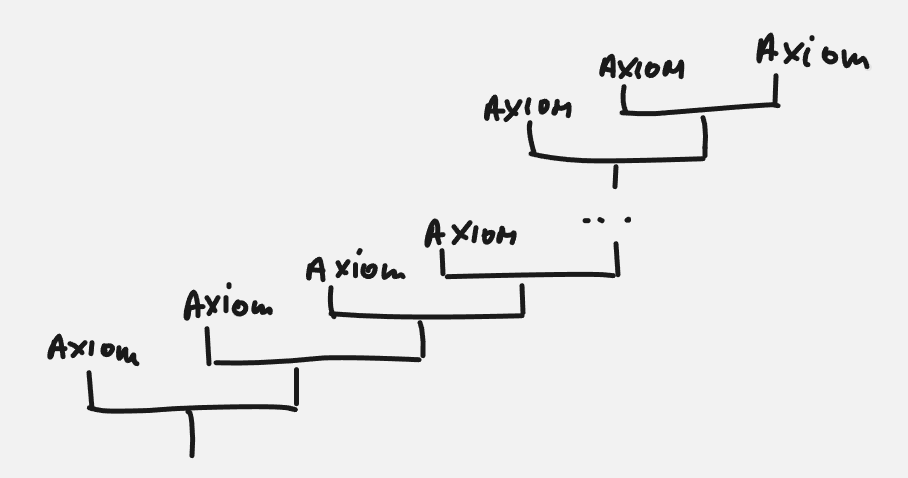
\includegraphics[scale=0.5]{treelook.png}\\
where all the branchings are made by the [$comp_{ns}^{!jump}$] rule, which in this case always separates one statement from the rest of the statement set.\\

\subsection{The beginning of the tree}
Beginning (root sub-tree) of the tree looks like this:\\
\\
\\
\begin{tiny}
\begin{prooftree}
        \Infer0[[$value_{ns}$]]{\tr{value\;step, s}{s1}}
        \Infer0[[$define_{ns}$]]{\tr{define, s1}{s2}}

        \Infer0[[$globalr_{ns}^{write}$]]{\tr{globalr, s2}{s3}}        
        \Infer0[]{...}        
        \Infer2[[$comp_{ns}^{!jump}$]]{\tr{P_2, s2}{s45}}

        \Infer2[[$comp_{ns}^{!jump}$]]{\tr{P_1, s1}{s45}}
        \Infer2[[$comp_{ns}^{!jump}$]]{\tr{P, s}{s45}}


\end{prooftree}
\end{tiny}\\
\\
\\
where $P$ is the whole program, $P_1$ is the whole program without the first statement (value step CRLF) and $P_2$ is the whole program without the first two statements (value step CRLF define CRLF), \\
s = (0,(0),(0,0,0),(),0,(,))\\
s1= (0,(step),(0,1,0),(),0,(,))\\
s2= (0,(0),(0,8,0),(step,F1,0),0,(,))\\
s45= (1,(0),(0,20,0),(step,F1,0),1,(,(4,2,1)))\\
\\

\subsection{The ending of the tree}
Ending (upper most leaf sub-tree) of the tree looks like this:\\
\\

\begin{tiny}
\begin{prooftree}
        \Infer0[[$jump_{ns}^{jump=0,0}$]]{\tr{jump, s42}{s43}}

        \Infer0[[$value_{ns}$]]{\tr{value\;0, s43}{s44}}        
        \Infer0[[$program_{ns}^{jump0}$]]{\tr{jump\;CRLF\;CRLF, s44}{s45}}        
        \Infer2[[$comp_{ns}^{!jump}$]]{\tr{value\;0\;CRLF\;jump\;CRLF\;CRLF, s43}{s45}}

        \Infer2[[$comp_{ns}^{!jump}$]]{\tr{jump\;CRLF\;value\;0\;CRLF\;jump\;CRLF\;CRLF, s42}{s45}}
        
        \Infer1[[$comp_{ns}^{!jump}$]]{...}
\end{prooftree}
\end{tiny}\\
\\
\\
where s42= (1,(-1),(0,17,0),(step,F1,0),0,(,(4,2,1)))\\
s43= (1,(0),(1,18,19),(step,F1,0),0,(,(4,2,1)))\\
s44= (1,(0),(0,19,0),(step,F1,0),0,(,(4,2,1)))\\
s45= (1,(0),(0,20,0),(step,F1,0),1,(,(4,2,1)))\\
\\


\subsection{The rest of the tree}
And here is what the tree can be filled in for the patter, described above.\\
\\
\textbf{All the leaves of the derivation tree:}\\
\begin{verbatim}
[programns_{ns}^{jump0}]
<jump CRLF CRLF, s44>->s45

[value_{ns}]
<value 0, s43>-> s44		

[jump_{ns}^{jump=0,0}]
<jump, s42>-> s43

[math exp3_{ns}]
<math ‘exp3’, s41>-> s42

[globalr_{ns}]
<globalr, s40>-> s41

[print_{ns}]
<print, s39>->s40

[globalr_{ns}]
<globalr, s38>-> s39

[globalw_{ns}]
<globalw, s37>->s38

[math exp1_{ns}]
<math ‘exp1’, s36>->s37

[globalr_{ns}]
<globalr, s35>-> s36

[call_{ns}]
<call, s34>-> s35

[value_{ns}]
<value step, s33>-> s34


[jump_{ns}^{jump=0,0}]
<jump, s32>-> s33


[math exp3_{ns}]
<math ‘exp3’, s31>-> s32


[globalr_{ns}]
<globalr, s30>-> s31


[print_{ns}]
<print, s29>->s30

[globalr_{ns}]
<globalr, s28>-> s29

[globalw_{ns}]
<globalw, s27>->s28

[math exp1_{ns}]
<math ‘exp1’, s26>->s27

[globalr_{ns}]
<globalr, s25>-> s26

[call_{ns}]
<call, s24>-> s25

[value_{ns}]
<value step, s23>-> s24

[jump_{ns}^{jump=0,0}]
<jump, s22>-> s23

[math exp3_{ns}]
<math ‘exp3’, s21>-> s22

[globalr_{ns}]
<globalr, s20>-> s21

[print_{ns}]
<print, s19>->s20

[globalr_{ns}]
<globalr, s18>-> s19

[globalw_ns]
<globalw, s17>->s18

[math_{ns}]
<math ‘exp1’, s16>->s17

[globalr_{ns}]
<globalr, s15>-> s16

[call_{ns}]
<call, s14>-> s15


[value_{ns}]
<value step, s13>->s14

[jump_{ns}^{jump=0,0}]
<jump, s12>-> s13

[math exp2_{ns}]
<math ‘exp2’, s11>->s12

[globalr_{ns}]
<globalr, s10>->s11

[globalw_{ns}]
<globalw, s9>-> s10

[value_{ns}]
<value 8, s2>-> s9

[define_{ns}]	
<define, s1>-> s2 

[value_{ns}] 
<value step,s> -> s1
\end{verbatim}

\textbf{Definitions for all states:}\\
\begin{verbatim}
    
F1 = (globalr CRLF math ‘exp1’ CRLF globalw CRLF globalr CRLF print CRLF)

s = (0,(0),(0,0,0),(),0,(,))
s1= (0,(step),(0,1,0),(),0,(,))
s2= (0,(0),(0,8,0),(step,F1,0),0,(,))
s9= (0,(8),(0,9,0),(step,F1,0),0,(,))
s10= (8,(0),(0,10,0),(step,F1,0),0,(,))
s11= (8,(8),(0,11,0),(step,F1,0),0,(,))
s12= (8,(-1),(0,12,0),(step,F1,0),0,(,))
s13= (8,(0),(1,13,13),(step,F1,0),0,(,))
s14= (8,(step),(0,14,0),(step,F1,0),0,(,))
s15= (8,(0),(0,15,0),(step,F1,0),0,(,))
s16= (8,(8),(0,15,0),(step,F1,0),0,(,))
s17= (8,(4),(0,15,0),(step,F1,0),0,(,))
s18= (4,(0),(0,15,0),(step,F1,0),0,(,))
s19= (4,(4),(0,15,0),(step,F1,0),0,(,))
s20= (4,(0),(0,15,0),(step,F1,0),0,(,(4)))
s21= (4,(4),(0,16,0),(step,F1,0),0,(,(4)))
s22= (4,(4),(0,17,0),(step,F1,0),0,(,(4)))
s23= (4,(0),(1,18,15),(step,F1,0),0,(,(4)))
s24= (4,(step),(0,15,0),(step,F1,0),0,(,(4)))
s25= (4,(0),(0,15,0),(step,F1,0),0,(,(4)))
s26= (4,(4),(0,15,0),(step,F1,0),0,(,(4)))
s27= (4,(2),(0,15,0),(step,F1,0),0,(,(4)))
s28= (2,(0),(0,15,0),(step,F1,0),0,(,(4)))
s29= (2,(2),(0,15,0),(step,F1,0),0,(,(4)))
s30= (2,(0),(0,15,0),(step,F1,0),0,(,(4,2)))
s31= (2,(2),(0,16,0),(step,F1,0),0,(,(4,2)))
s32= (2,(4),(0,17,0),(step,F1,0),0,(,(4,2)))
s33= (2,(0),(1,18,15),(step,F1,0),0,(,(4,2)))
s34= (2,(step),(0,15,0),(step,F1,0),0,(,(4,2)))
s35= (2,(0),(0,15,0),(step,F1,0),0,(,(4,2)))
s36= (2,(2),(0,15,0),(step,F1,0),0,(,4,2))
s37= (2,(1),(0,15,0),(step,F1,0),0,(,4,2))
s38= (1,(0),(0,15,0),(step,F1,0),0,(,4,2))
s39= (1,(2),(0,15,0),(step,F1,0),0,(,4,2))
s40= (1,(0),(0,15,0),(step,F1,0),0,(,(4,2,1)))
s41= (1,(1),(0,16,0),(step,F1,0),0,(,(4,2,1)))
s42= (1,(-1),(0,17,0),(step,F1,0),0,(,(4,2,1)))
s43= (1,(0),(1,18,19),(step,F1,0),0,(,(4,2,1)))
s44= (1,(0),(0,19,0),(step,F1,0),0,(,(4,2,1)))
s45= (1,(0),(0,20,0),(step,F1,0),1,(,(4,2,1)))
\end{verbatim}


\end{document}
